\documentclass[12pt, twoside]{article}
\usepackage[letterpaper, margin=1in, headsep=0.2in]{geometry}
\setlength{\headheight}{0.6in}
%\usepackage[english]{babel}
\usepackage[utf8]{inputenc}
\usepackage{microtype}
\usepackage{amsmath}
\usepackage{amssymb}
%\usepackage{amsfonts}
\usepackage{siunitx} %units in math. eg 20\milli\meter
\usepackage{yhmath} % for arcs, overparenth command
\usepackage{tikz} %graphics
\usetikzlibrary{quotes, angles}
\usepackage{graphicx} %consider setting \graphicspath{{images/}}
\usepackage{parskip} %no paragraph indent
\usepackage{enumitem}
\usepackage{multicol}
\usepackage{venndiagram}

\usepackage{fancyhdr}
\pagestyle{fancy}
\fancyhf{}
\renewcommand{\headrulewidth}{0pt} % disable the underline of the header
\raggedbottom
\hfuzz=2mm %suppresses overfull box warnings

\usepackage{hyperref}

\fancyhead[LE]{\thepage}
\fancyhead[RO]{\thepage \\ Name: \hspace{4cm} \,\\}
\fancyhead[LO]{BECA / Dr. Huson / Geometry\\*  Unit 6: Analytic geometry\\* 6 January 2023}

\begin{document}

\subsubsection*{6.9 Classwork: Applications of systems of linear equations \hfill HSG.REI.C.6}
\begin{enumerate}
\item Two values, $x$ and $y$, have a total of 12. The larger, $y$, is 3 more than twice $x$. Write a system of linear equations to represent this situation, then graph them to solve.
\begin{flushright}
  \begin{tikzpicture}[scale=.65]
    \draw [help lines] (0,0) grid (12,12);
    \draw [thick, ->] (0,0) -- (12.4,0) node [above right] {$x$};
    \draw [thick, ->] (0,0)--(0,12.4) node [right] {$y$};
    \foreach \x in {1,...,12}
    \draw[shift={(\x,0)}] (0pt,-3pt)--(0pt,3pt) node[below=5pt] {$\x$};
    \foreach \y in {1,...,12}
    \draw[shift={(0,\y)}] (-3pt,0pt)--(3pt,0pt) node[left=5pt] {$\y$};
  \end{tikzpicture}
  \end{flushright}

\item Steve buys eight sandwiches for his friends. Small sandwiches cost \$3 and large ones \$6. He spends \$33 in all. How many of each kind did he buy?
\begin{flushright}
  \begin{tikzpicture}[scale=.65]
    \draw [help lines] (0,0) grid (12,12);
    \draw [thick, ->] (0,0) -- (12.4,0) node [above right] {$x$};
    \draw [thick, ->] (0,0)--(0,12.4) node [right] {$y$};
    \foreach \x in {1,...,12}
    \draw[shift={(\x,0)}] (0pt,-3pt)--(0pt,3pt) node[below=5pt] {$\x$};
    \foreach \y in {1,...,12}
    \draw[shift={(0,\y)}] (-3pt,0pt)--(3pt,0pt) node[left=5pt] {$\y$};
  \end{tikzpicture}
  \end{flushright}

\newpage
\item Graph and label the two equations. Mark their intersection as an ordered pair.
  \begin{multicols}{2}
    $f(x) = -\frac{1}{2}x+3$ \\
    $g(x) = \frac{7}{4}x-6$
  \end{multicols}  \vspace{1cm}
  Are the lines parallel, perpendicular, or neither? Justify your answer.
  \vspace{1.5cm}
  \begin{center}
  \begin{tikzpicture}[scale=.635]
    \draw [help lines] (-10,-8) grid (10,10);
    \draw [thick, ->] (-10.2,0) -- (10.4,0) node [below right] {$x$};
    \draw [thick, ->] (0,-8.2)--(0,10.4) node [left] {$y$};
  \end{tikzpicture}
  \end{center}


\end{enumerate}
\end{document}